\documentclass[border=6pt]{standalone}
\usepackage{tikz}
\usetikzlibrary{arrows.meta,positioning,decorations.pathreplacing,calc}
\begin{document}
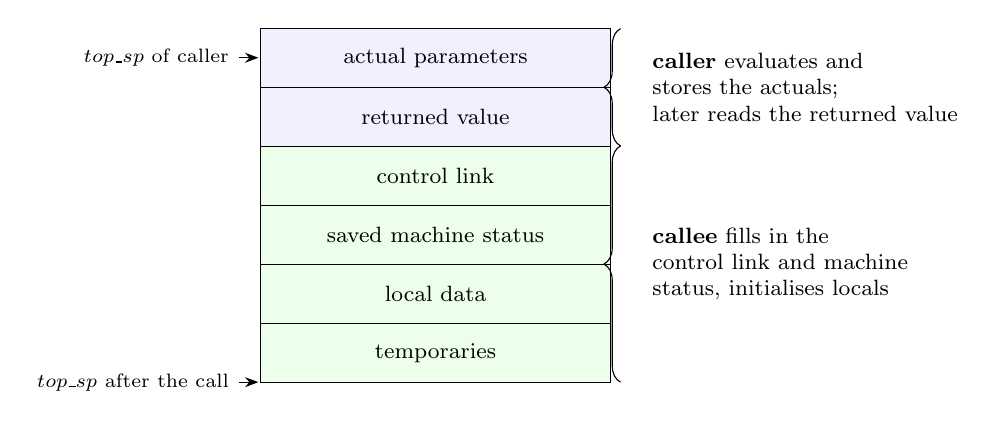
\begin{tikzpicture}[>=Stealth,font=\small,
  cell/.style={draw,minimum width=4.4cm,text width=4.2cm,minimum height=0.75cm,align=center,font=\footnotesize}]
\node[cell,fill=blue!6] (c1) at (0,0)    {actual parameters};
\node[cell,fill=blue!6] (c2) at (0,-0.75) {returned value};
\node[cell,fill=green!8] (c3) at (0,-1.5) {control link};
\node[cell,fill=green!8] (c4) at (0,-2.25) {saved machine status};
\node[cell,fill=green!8] (c5) at (0,-3.0) {local data};
\node[cell,fill=green!8] (c6) at (0,-3.75) {temporaries};
\draw[decorate,decoration={brace,amplitude=6pt,mirror}] (2.35,0.37) -- node[right=8pt,align=left,font=\footnotesize] {\textbf{caller} evaluates and\\ stores the actuals;\\ later reads the returned value} (2.35,-1.12);
\draw[decorate,decoration={brace,amplitude=6pt,mirror}] (2.35,-1.12) -- node[right=8pt,align=left,font=\footnotesize] {\textbf{callee} fills in the\\ control link and machine\\ status, initialises locals} (2.35,-4.12);
\node[font=\scriptsize,anchor=east] at (-2.5,0) {$top\_sp$ of caller};
\draw[->] (-2.5,0) -- (-2.25,0);
\node[font=\scriptsize,anchor=east] at (-2.5,-4.12) {$top\_sp$ after the call};
\draw[->] (-2.5,-4.12) -- (-2.25,-4.12);
\end{tikzpicture}
\end{document}
